\documentclass[a4paper, 12pt]{article}
 % This is used for setting the margins
\usepackage[top=1in, bottom=1in, left=1in, right=1in]{geometry}

%%%% IMPORTED PACKAGES %%%
\usepackage{graphicx}
\usepackage{amsmath}
% Important when citations include URLs.
\usepackage[pdftex]{hyperref}
%%%%%%%%%%%%%%%%%%%%%%%%%%

\newenvironment{keywords}
{\begin{list}{}{\setlength{\leftmargin}{1em}}\item[\hskip\labelsep \bfseries Keywords:]}
{\end{list}}

\begin{document}

%%%%%%%% COVER %%%%%%%%%%%
\begin{titlepage}
\begin{center}
	\vspace{5 mm}
	    \textbf{\Large TECHNICAL UNIVERSITY OF MADRID}
	\par
	\vspace{10 mm}
	\begin{figure}[htb]
	    \centering
	    
\includegraphics[scale=0.7]{images/general/uni-logo.png}
	\end{figure}

    %\vspace{10 mm}\textbf{\large \degree} \par
    %\vspace{10 mm}\textbf{\large \faculty} \par
    %\vspace{20 mm}\textbf{\large \department } \par


    \vspace{20 mm}\textsc{\Large Analysis of Spanish COVID-19 tracking apps}
    \par
    \vspace{10 mm}\textsc{I\&E Seminars: Digital Health}
    \par
    \vspace{10 mm}
    \textsc{
        AUTHOR: \\
        Cristian M. Abrante Dorta
    }
    \par
	\rule{80mm}{0.1mm}\\
	\vspace{10 mm}
	
    \vspace*{\stretch{2}}
    \textsc{EIT Digital Master's degree in Data Science}\\
    \textsc{\today}
\end{center}
\end{titlepage}

%%%%%%%%%%%%%%%%%%%%%%%%%%

%%%%%% ABSTRACT %%%%%%%%%%
\newpage
\begin{abstract}
{\em

Lorem ipsum dolor sit amet, consectetur adipiscing elit. Nulla quis maximus dui. Sed congue ultrices diam, ac posuere orci vehicula sit amet. Sed eu iaculis ex. Vestibulum tempor dictum nunc, sed tincidunt tortor feugiat a. Quisque cursus ut leo ac fringilla. Nullam feugiat, est quis egestas faucibus, nulla diam cursus justo, in dapibus lorem ipsum nec augue. Proin mattis fringilla lectus aliquet congue.

\bigskip

Nulla orci augue, convallis sit amet neque et, vehicula tincidunt dolor. Vivamus commodo massa sit amet lobortis blandit. Curabitur imperdiet mi nec elit porttitor dictum. Vestibulum in urna risus. In ac laoreet lorem. Donec in libero eu dolor iaculis ullamcorper sit amet sit amet velit. Phasellus sit amet felis purus. Integer pretium nec erat quis sagittis. Etiam dictum hendrerit venenatis. Vestibulum semper, odio non efficitur suscipit, lorem ex iaculis libero, id pretium lacus augue a ipsum. Suspendisse commodo sed justo sit amet pharetra. Donec interdum pulvinar molestie. Class aptent taciti sociosqu ad litora torquent per conubia nostra, per inceptos himenaeos.
}

\begin{keywords}
Keyword 1, Keyword 2, Keyword 3
\end{keywords}
\end{abstract}

\newpage{\pagestyle{empty}}
\thispagestyle{empty}

%%%%%%%%%%%%%%%%%%%%%%%%%%

%% TABLE OF CONTENTS %%%%%
\tableofcontents
\newpage{\pagestyle{empty}}

%%%%%%%%%%%%%%%%%%%%%%%%%%

%%% Set the counter of the page to 1 after the index.
\setcounter{page}{1}

%%%%%%%% INTRODUCTION %%%%%%%
\section{Introduction}
\label{section:introduction}

The COVID-19 pandemic have caused a huge impact all over the world. The consequences of this pandemic are going to be cross-sectional, affecting both the economical development of many regions but also it is going to change the social behaviour in deep level. In this sense, also the healthcare systems have to be re-think and adapted for this new situation, taking into account that in the future this could happen again. \\

Focusing on healthcare applications, in the past they have been really effective at different levels. They have been used by patients that want to consult their electronic medical records, and also that want to appoint a date with a doctor. During this pandemic, many governments and institutions have taken into account the possibilities of generating a pandemic.

%%%%%%%%%%%%%%%%%%%%%%%%%%

%%%%%%%% SECTION 2 %%%%%%%
\section{Review of the current COVID-19 applications and websites}
\label{section:review}

In this section it is covered the different approaches that many countries, businesses and institutions are following for the development of applications related to the COVID-19 pandemic. Specially focusing on the case of Spain, where many applications have been developed both at regional and general level.

\subsection{Information and auto diagnosis solutions}

Information and auto-diagnosis applications and websites are the first approaches that many regions have followed for the development of software that could help to fight the pandemic. The main aim of those software products is to offer a reliable source of information and at the same time decongest telephone lines that are offered for citizens. \\

In Spain, the central source of information for the pandemic has been the website of the Ministry of Health \cite{ministerio-sanidad}. In this website is where it is published the scientific information regarding the disease, and also is where the official numbers of new infected, dead and tested population is published every day.\\

As the public health in Spain is decentralized, each autonomous community or region (Comunidad Autónoma in Spanish), have all the competencies for the organization of hospitals and logistics of healthcare in the region. This has caused some of them to have developed specific applications for auto-diagnosis and also for giving specific information to the citizens of the region. In this analysis, it is covered the solutions proposed by the community of Madrid, and the community of Catalonia, the two most affected regions in the country, and also the solution proposed by the central government.

\paragraph{CoronaMadrid} \mbox{}\\

As Madrid is the most affected region of Spain, the development of an application that could help the healthcare system to resist the pandemic was a critical task. \textit{CoronaMadrid} \cite{coronamadrid-page} was one of the first applications developed in Spain regarding the pandemic; it consists in a website and an application for Android and iOS that offers the possibility of filling a self-diagnosis form, and then a classification system would determine if you have enough significant symptoms for being considered as a COVID-19 affected. In the beginning, this application was permissive, offering the possibility of doing the diagnosis test without introducing any personal information, but nowadays this policy has changed and the user should introduce their name, personal ID, and direction in the Madrid community. This change was done to improve the reliability of the data that was collected \cite{coronamadrid-privacy}. \\

\begin{figure}[!htb]
   \begin{minipage}{0.33\textwidth}
     \centering
     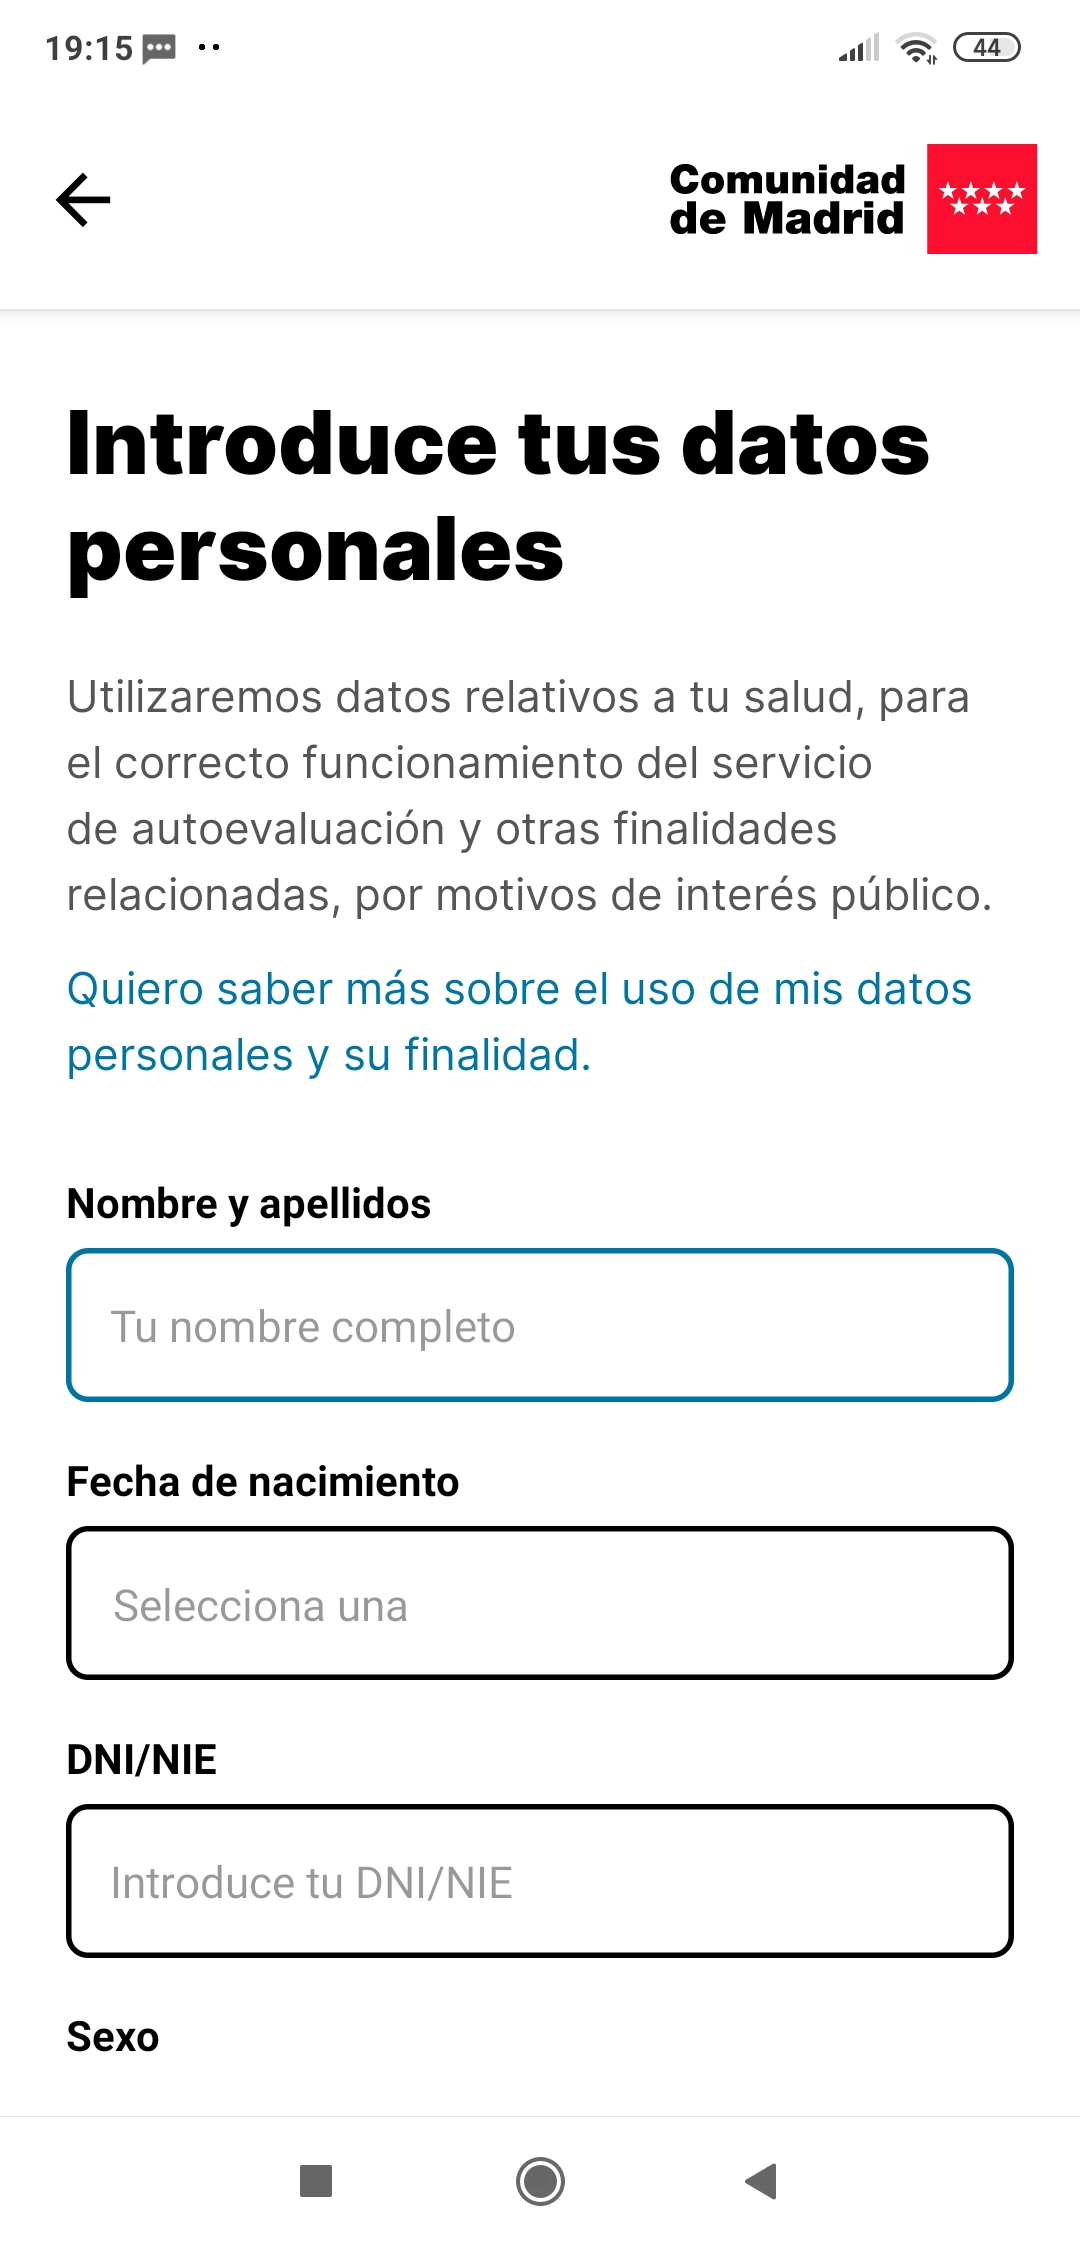
\includegraphics[scale=0.06]{images/discussion/coronamadrid-1.jpg}
   \end{minipage}\hfill
   \begin{minipage}{0.33\textwidth}
     \centering
     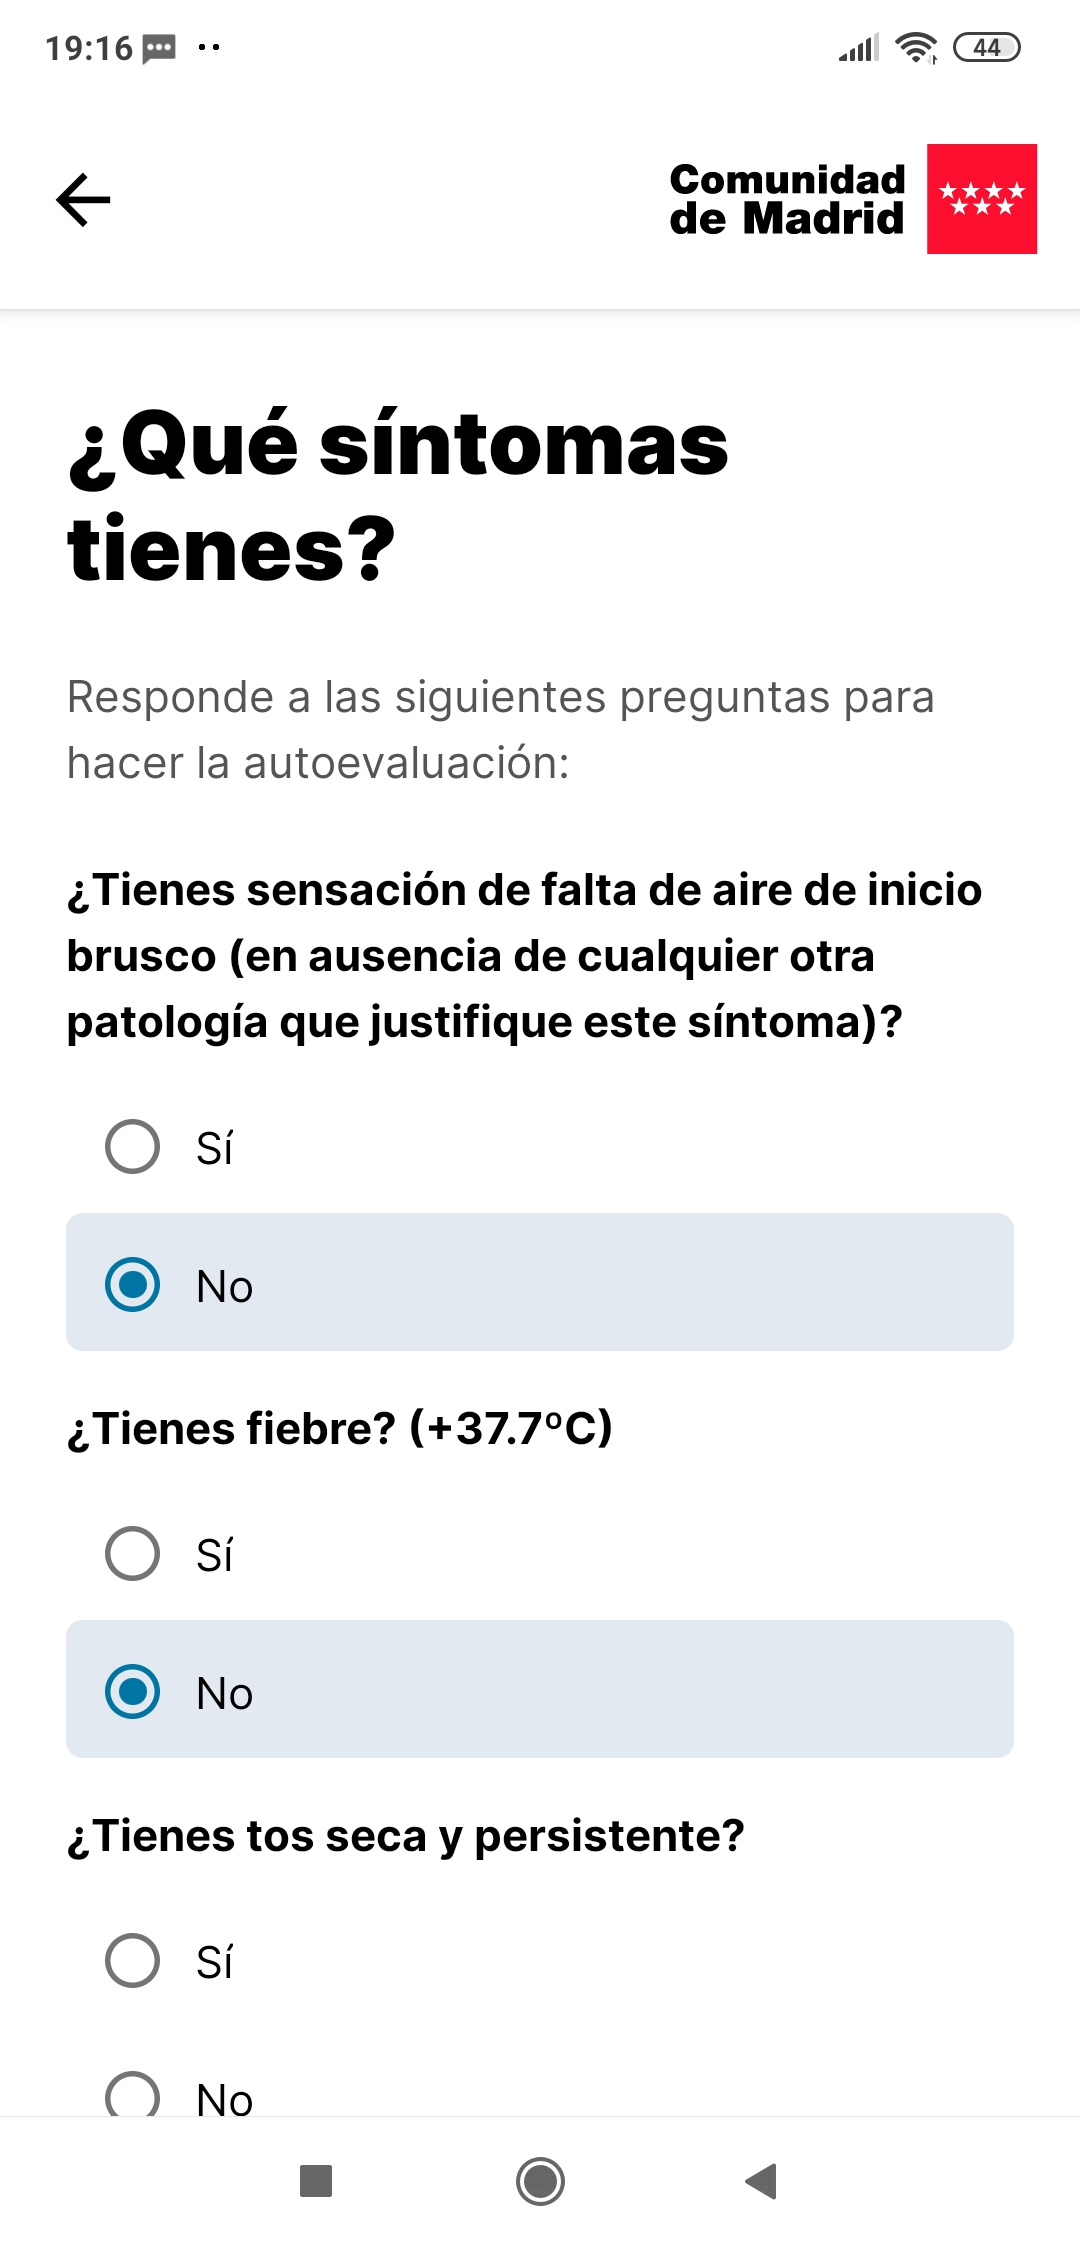
\includegraphics[scale=0.06]{images/discussion/coronamadrid-2.jpg}
   \end{minipage}
   \begin{minipage}{0.33\textwidth}
     \centering
     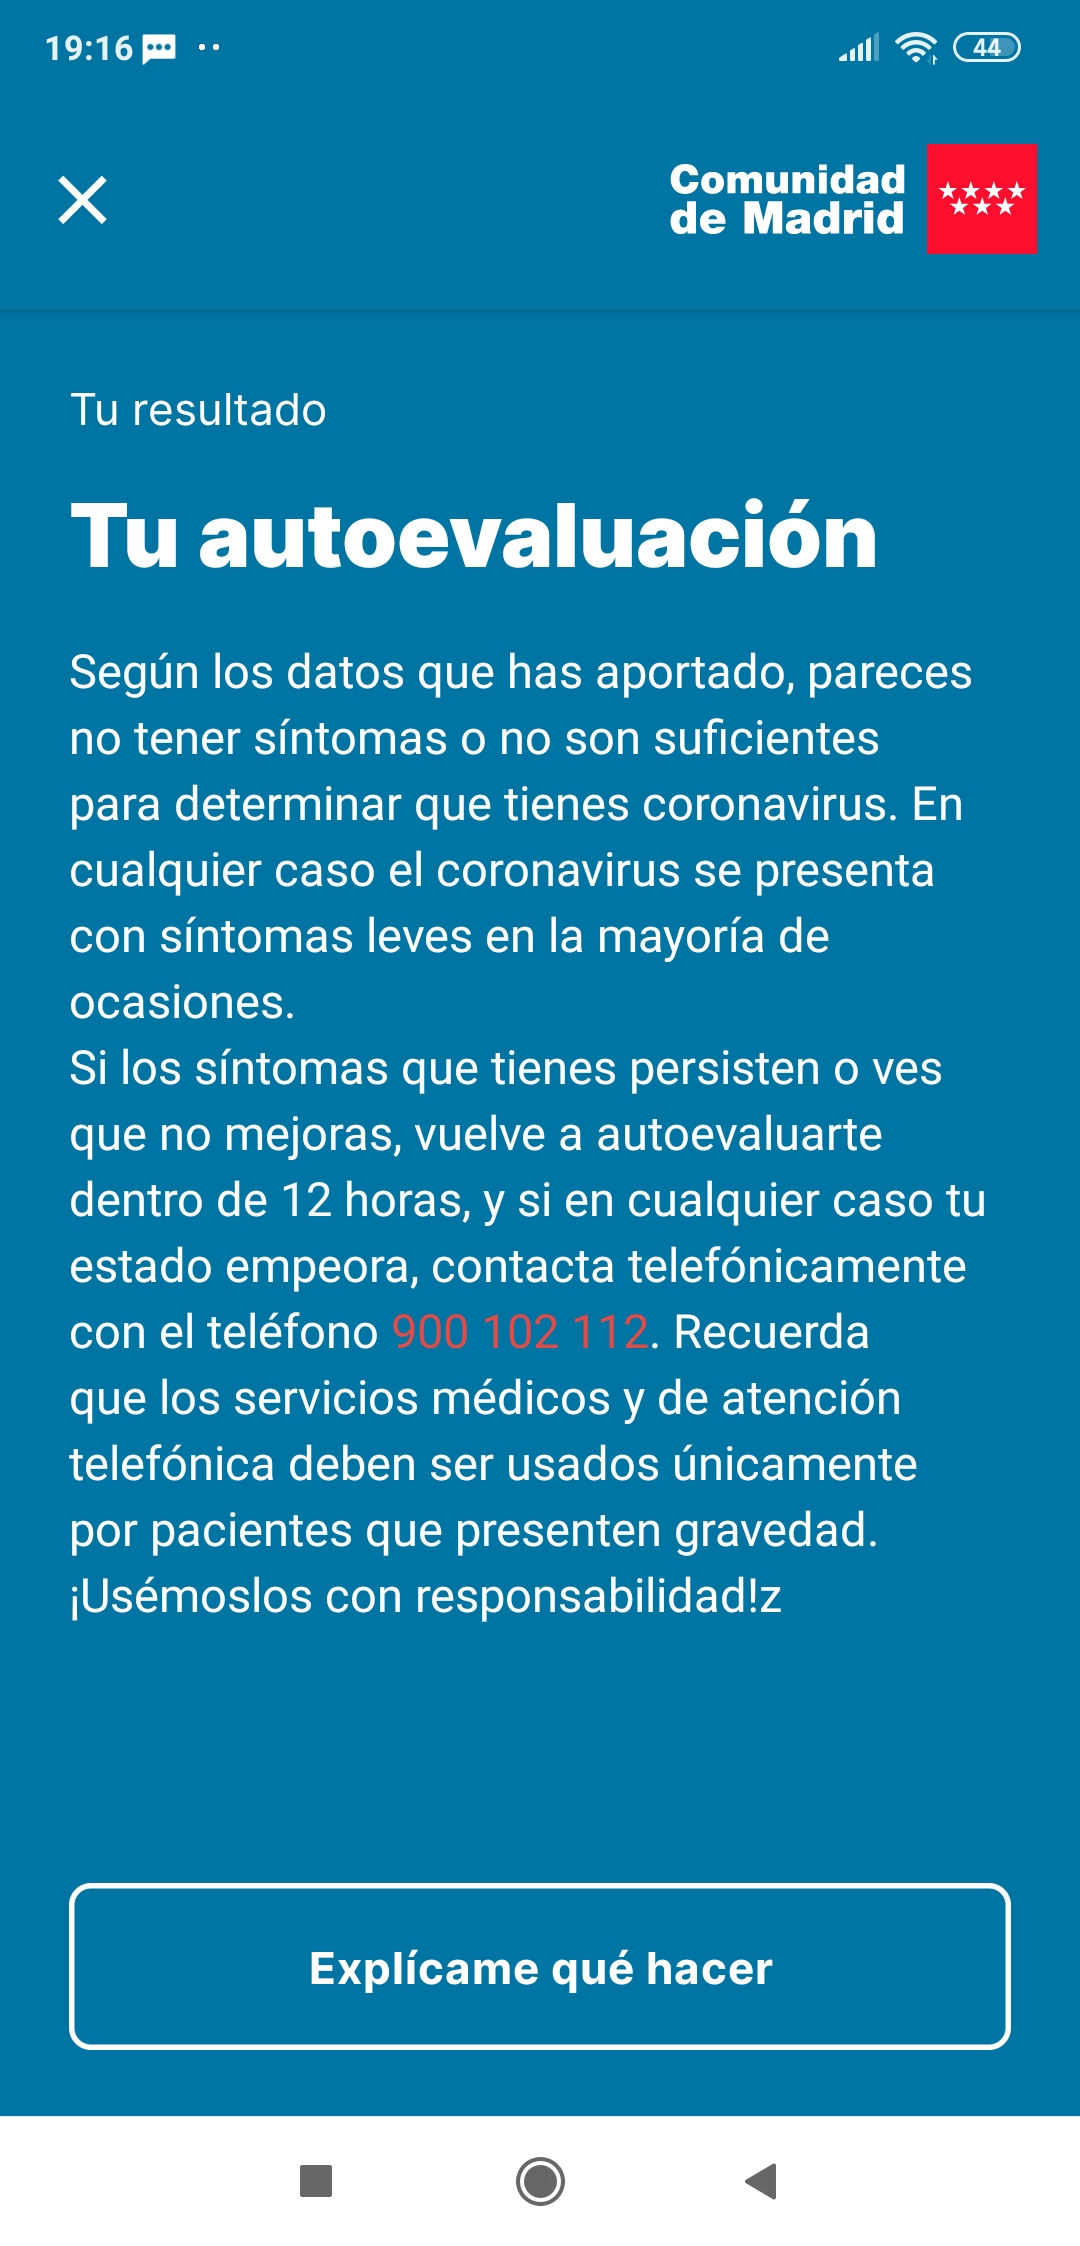
\includegraphics[scale=0.06]{images/discussion/coronamadrid-3.jpg}
   \end{minipage}
   \caption{Different screens of the application CoronaMadrid}
   \label{fig:coronamadrid}
\end{figure}

Analyzing the visual components and user experience of the application (Some screenshots of the Android app are shown in Figure \ref{fig:coronamadrid}), it consists of a simple form where the user introduces the personal details in the beginning, and then answer several questions successively in each screen. After that process, the application gives a result, showing the actuation protocol in case it is needed. The application is characterized by its simplicity, which makes it accessible for all types of users.

\paragraph{STOP COVID19 CAT} \mbox{} \\

It is also remarkable the impact of the COVID-19 pandemic in the region of Catalonia, being the second community in the number of deaths and total infected population. This situation pushed this community to follow Madrid in the development of an information application \cite{first-covid19-apps}, centered on the Catalonia region. The name of the application is STOP COVID19 CAT \cite{stop-covid19-cat}, and it was developed by the Generalitat de Catalunya (Government of Catalonia). The operation of the application is very similar to \textit{CoronaMadrid}, with a specific form which performs an auto-diagnosis test. In the field of data consistency, the main difference between them is that this application asks for the ID number of the sanitary card, and did not ask for the direction within the community, which is directly obtained from the GPS of the device. \\

\begin{figure}[!htb]
   \begin{minipage}{0.33\textwidth}
     \centering
     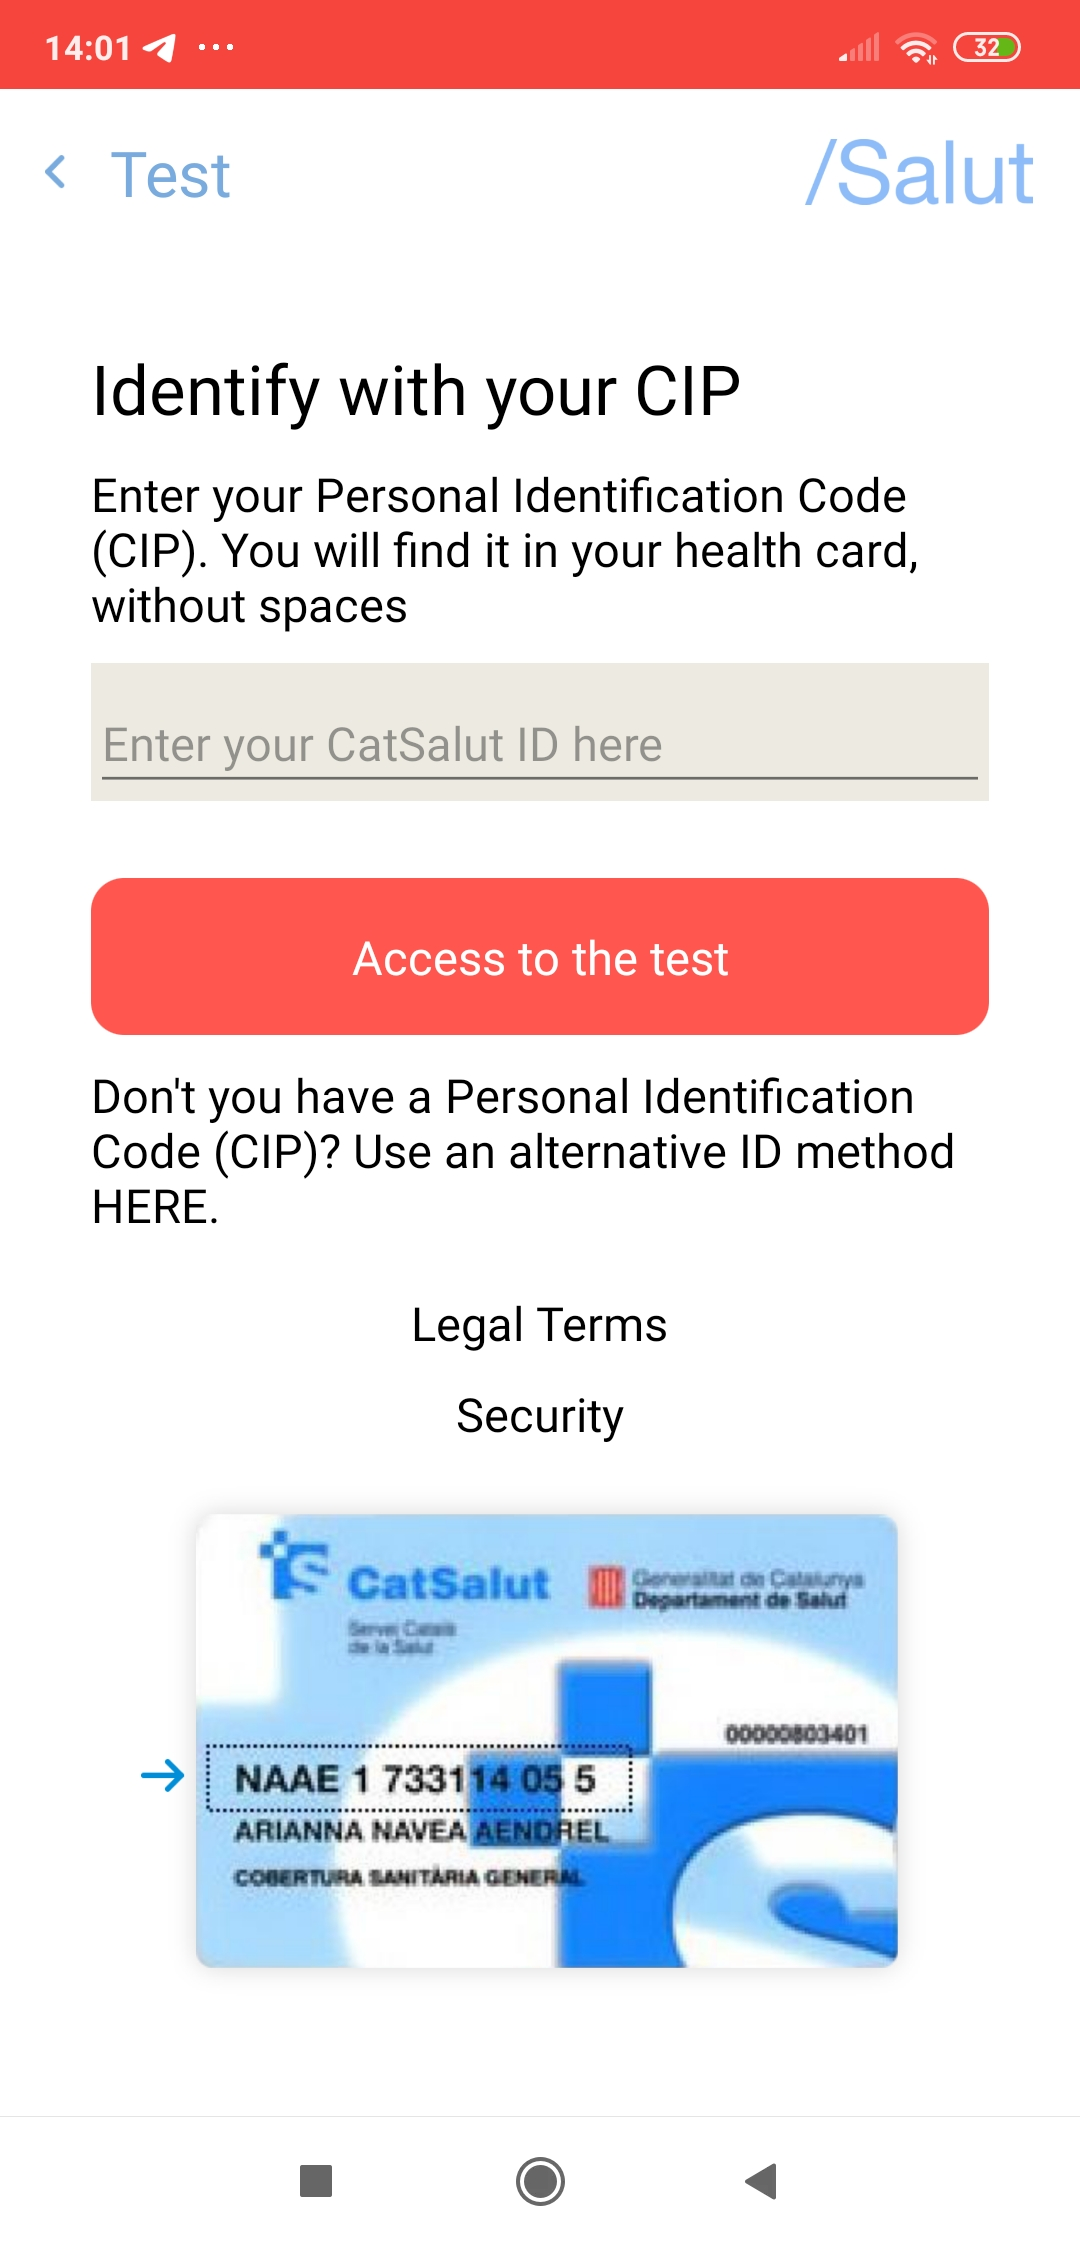
\includegraphics[scale=0.06]{images/discussion/covid-cat-1.jpg}
   \end{minipage}\hfill
   \begin{minipage}{0.33\textwidth}
     \centering
     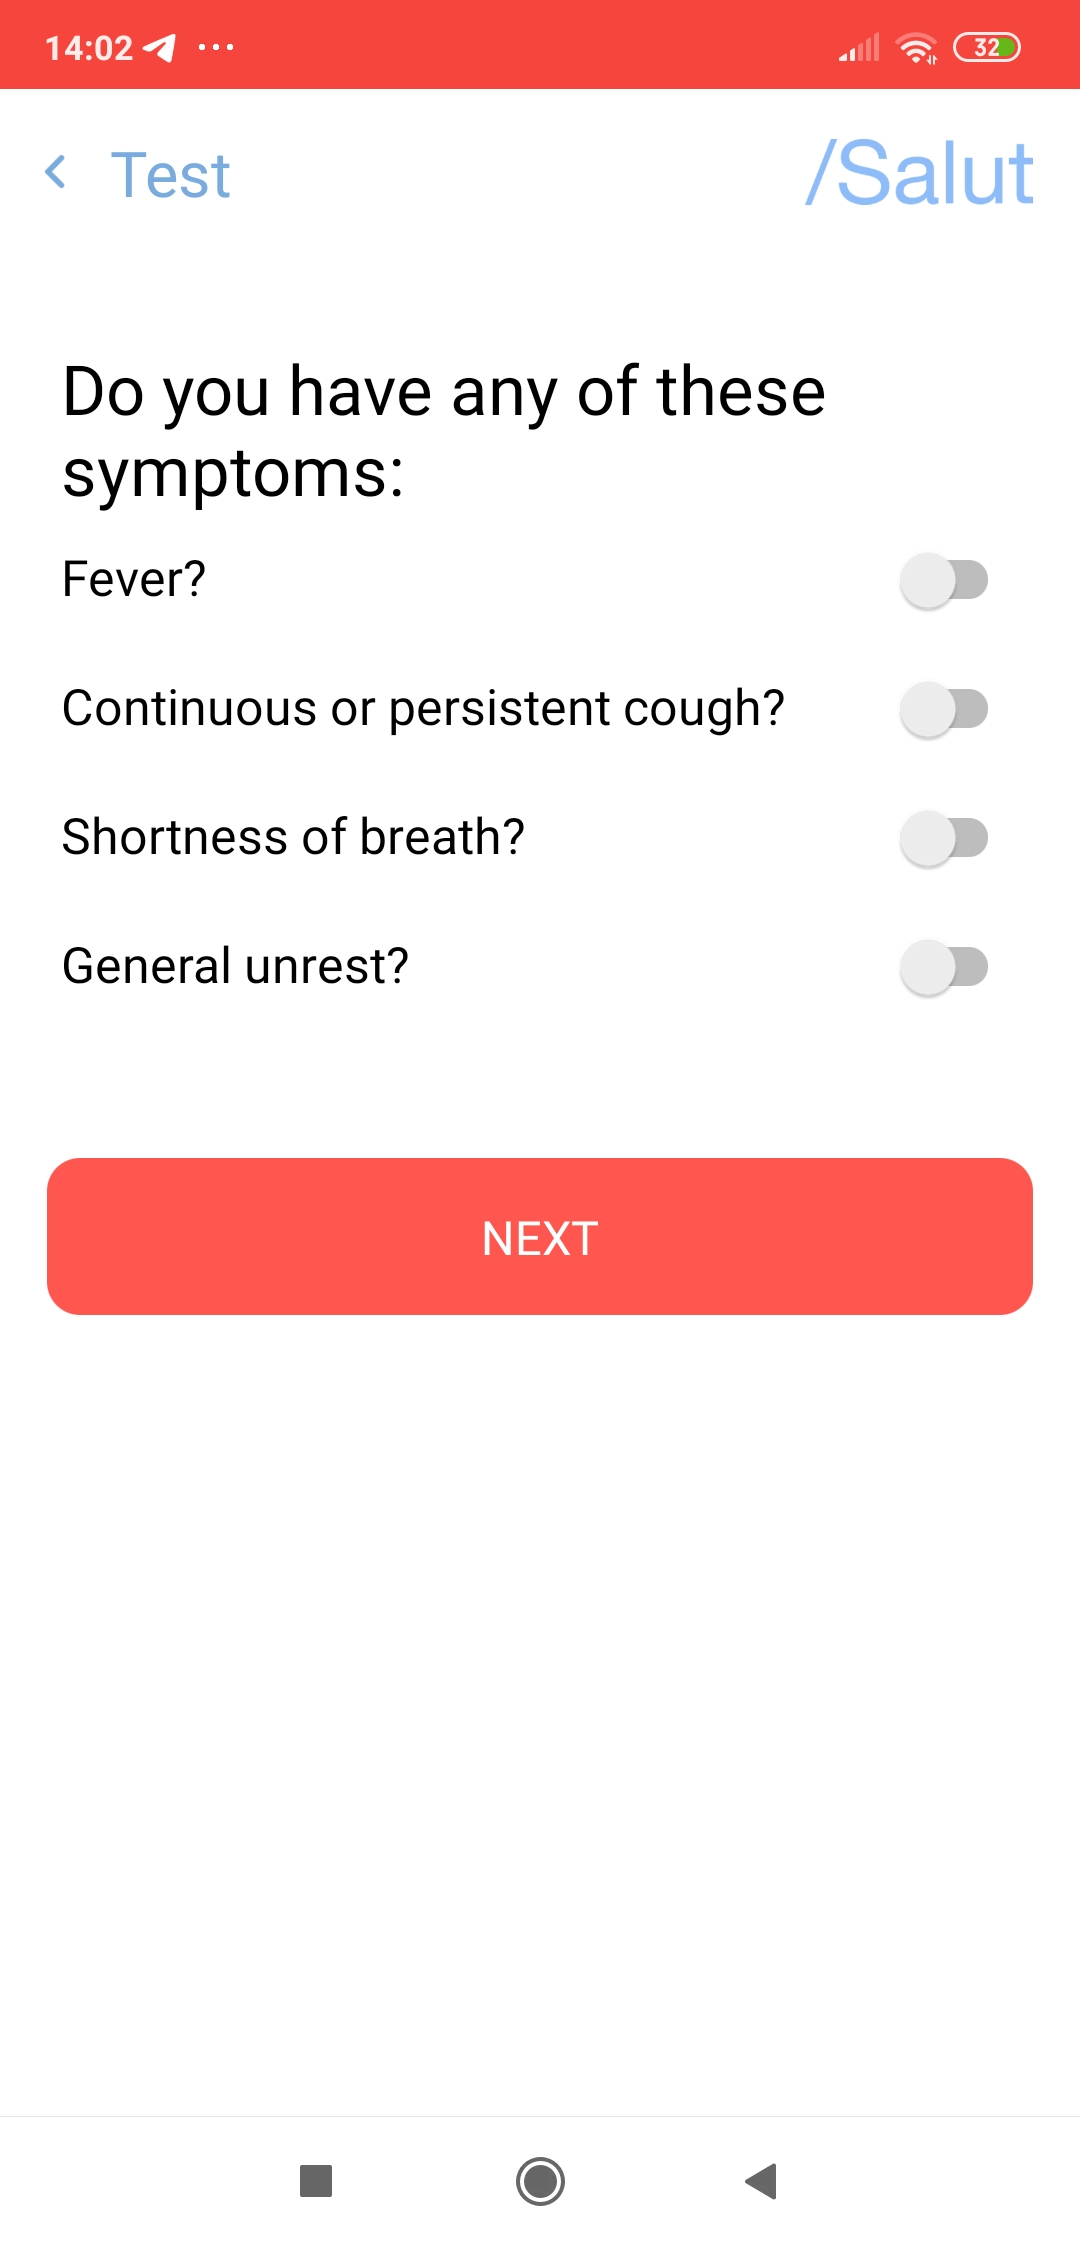
\includegraphics[scale=0.06]{images/discussion/covid-cat-2.jpg}
   \end{minipage}
   \begin{minipage}{0.33\textwidth}
     \centering
     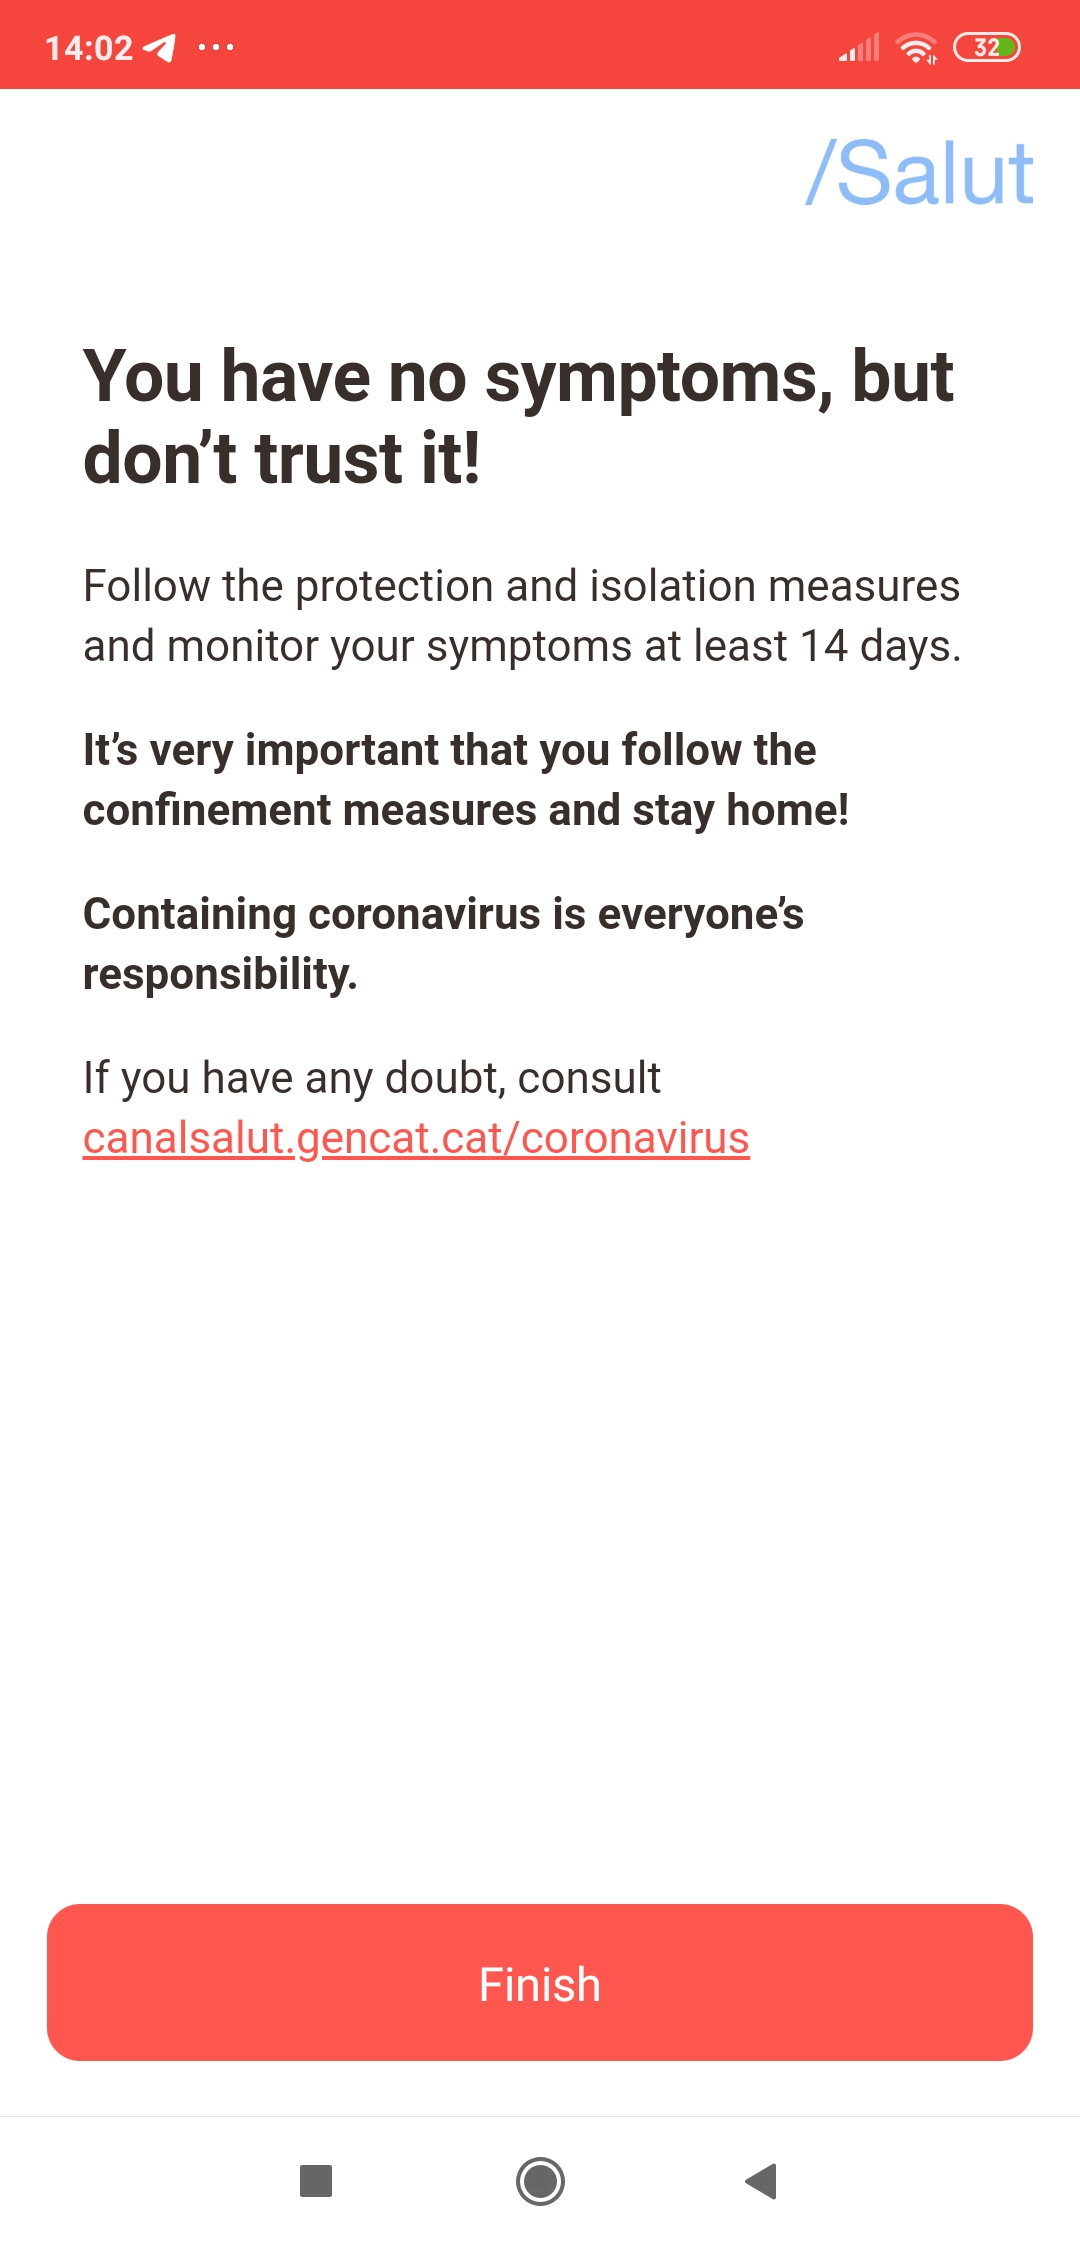
\includegraphics[scale=0.06]{images/discussion/covid-cat-3.jpg}
   \end{minipage}
   \caption{Different screens of the application STOP COVID19 CAT}
   \label{fig:covid-cat}
\end{figure}

Speaking about user experience, STOP COVID19 CAT has a worse performance. The display of the information is less intuitive, mainly because of the use of switches instead of radio buttons, as shown in Figure \ref{fig:covid-cat}. Another significant difference is that the Catalonia app allows us to do as many auto evaluations as we want, and \textit{CoronaMadrid} only allows users to do the evaluation once per day. This control over the frequency improves the reliability of the data collected. 

\paragraph{Asistencia COVID-19} \mbox{} \\

As \textit{CoronaMadrid} was the first auto diagnosis application of the virus in Spain, when the government wanted to do a central version that will be used as a substitute for the ones developed in the autonomous communities, the logic path will be to copy the main functionalities of it. The application developed by the National Department of digitization and artificial intelligence (\textit{Secretaría de Estado de digitalización e inteligencia artificial} in Spanish), was called Asistencia COVID-19. The way that these application works is really similar in how \textit{CoronaMadrid} works, especially in the data that is recollected: name, national ID number, direction, and autonomous community where you are located. Also it requires the activation of the GPS service in the device, which has caused some social controversy \cite{geolocalization-asistencia-covid-19}. It is important to mention that the operability of this application is limited to some regions, initially it was developed for Madrid, but now it has been extended to five additional communities.\\

\begin{figure}[!htb]
   \begin{minipage}{0.33\textwidth}
     \centering
     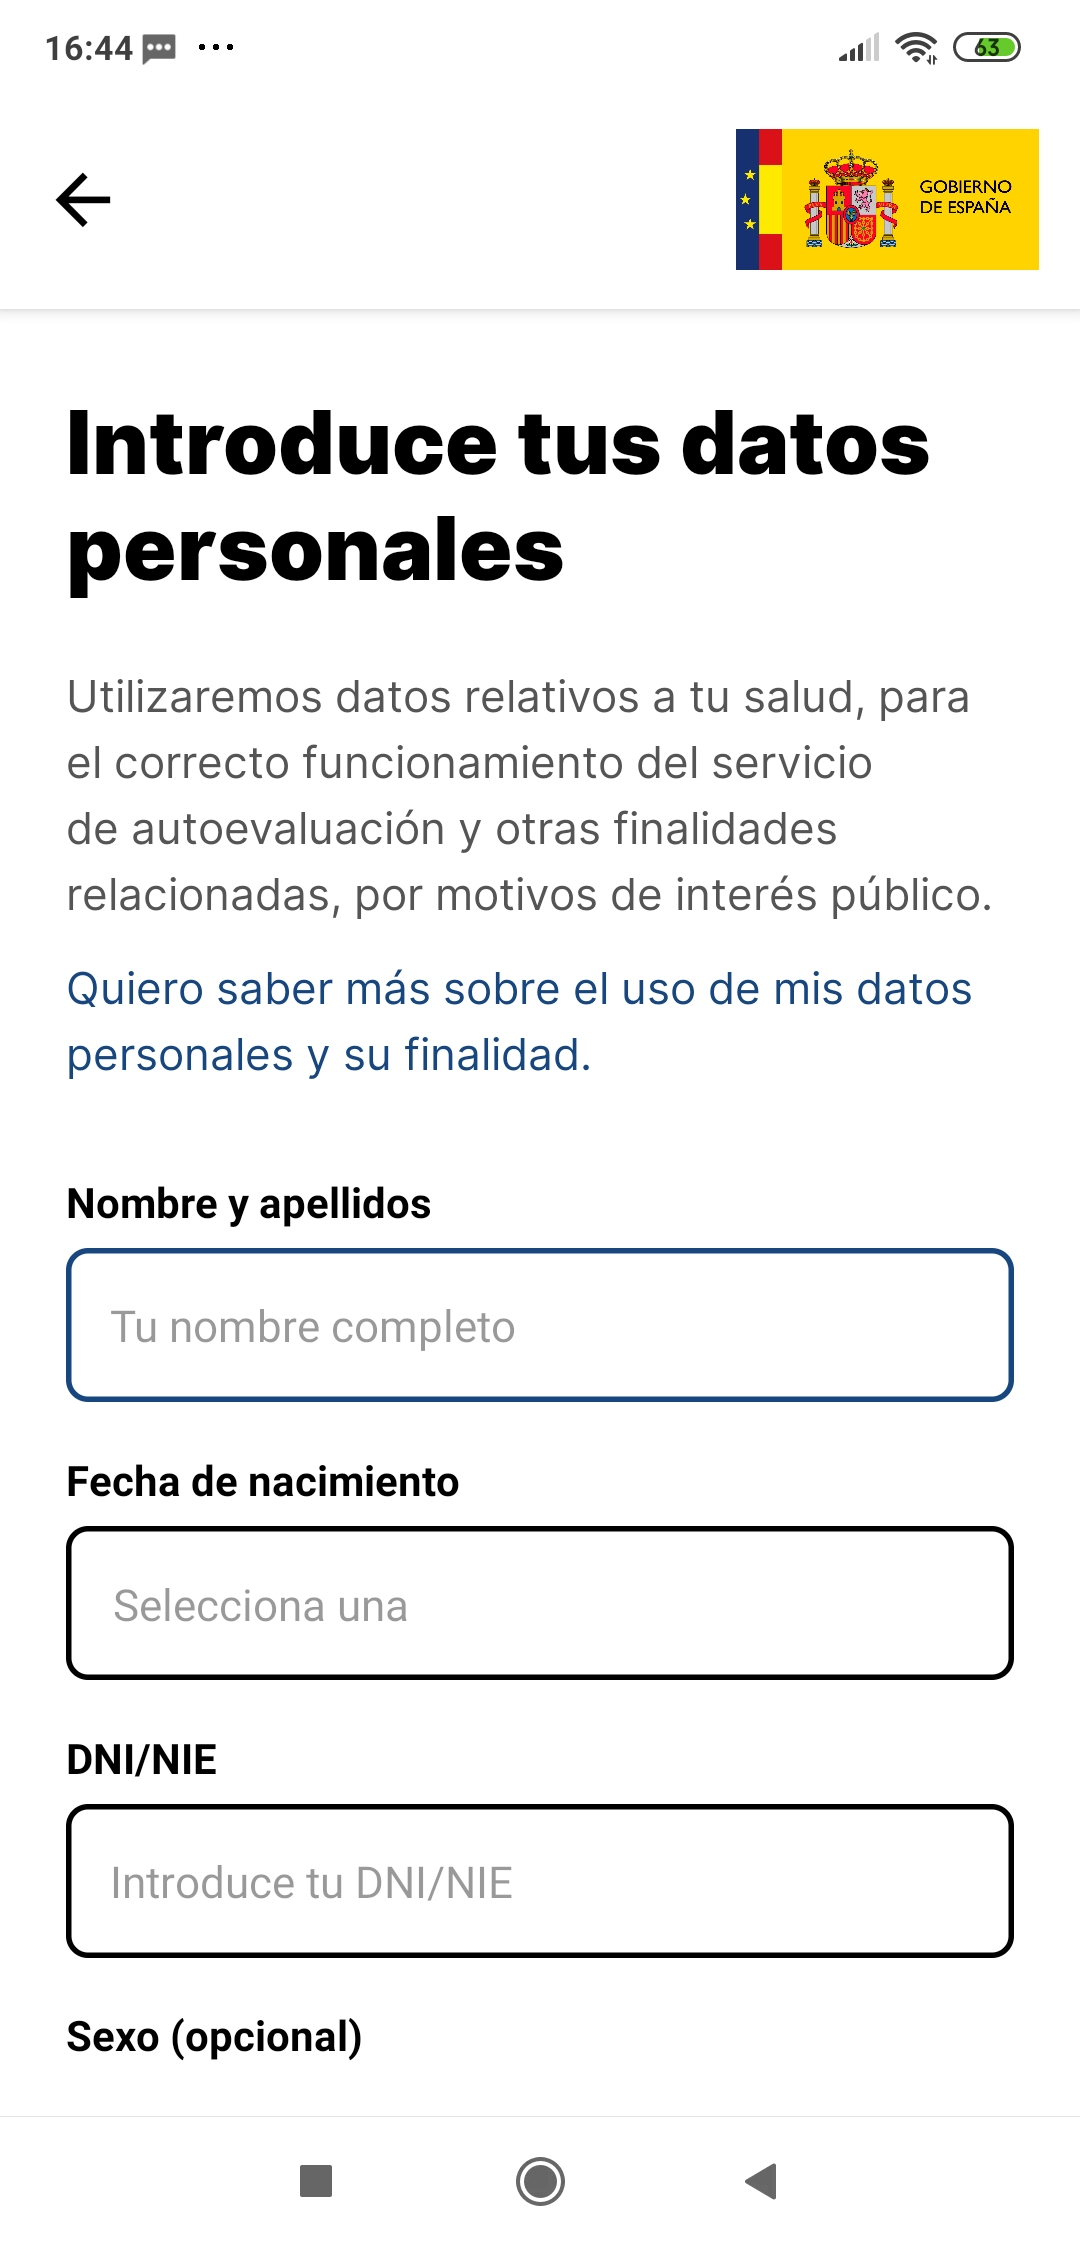
\includegraphics[scale=0.06]{images/discussion/asistencia-covid-1.jpg}
   \end{minipage}\hfill
   \begin{minipage}{0.33\textwidth}
     \centering
     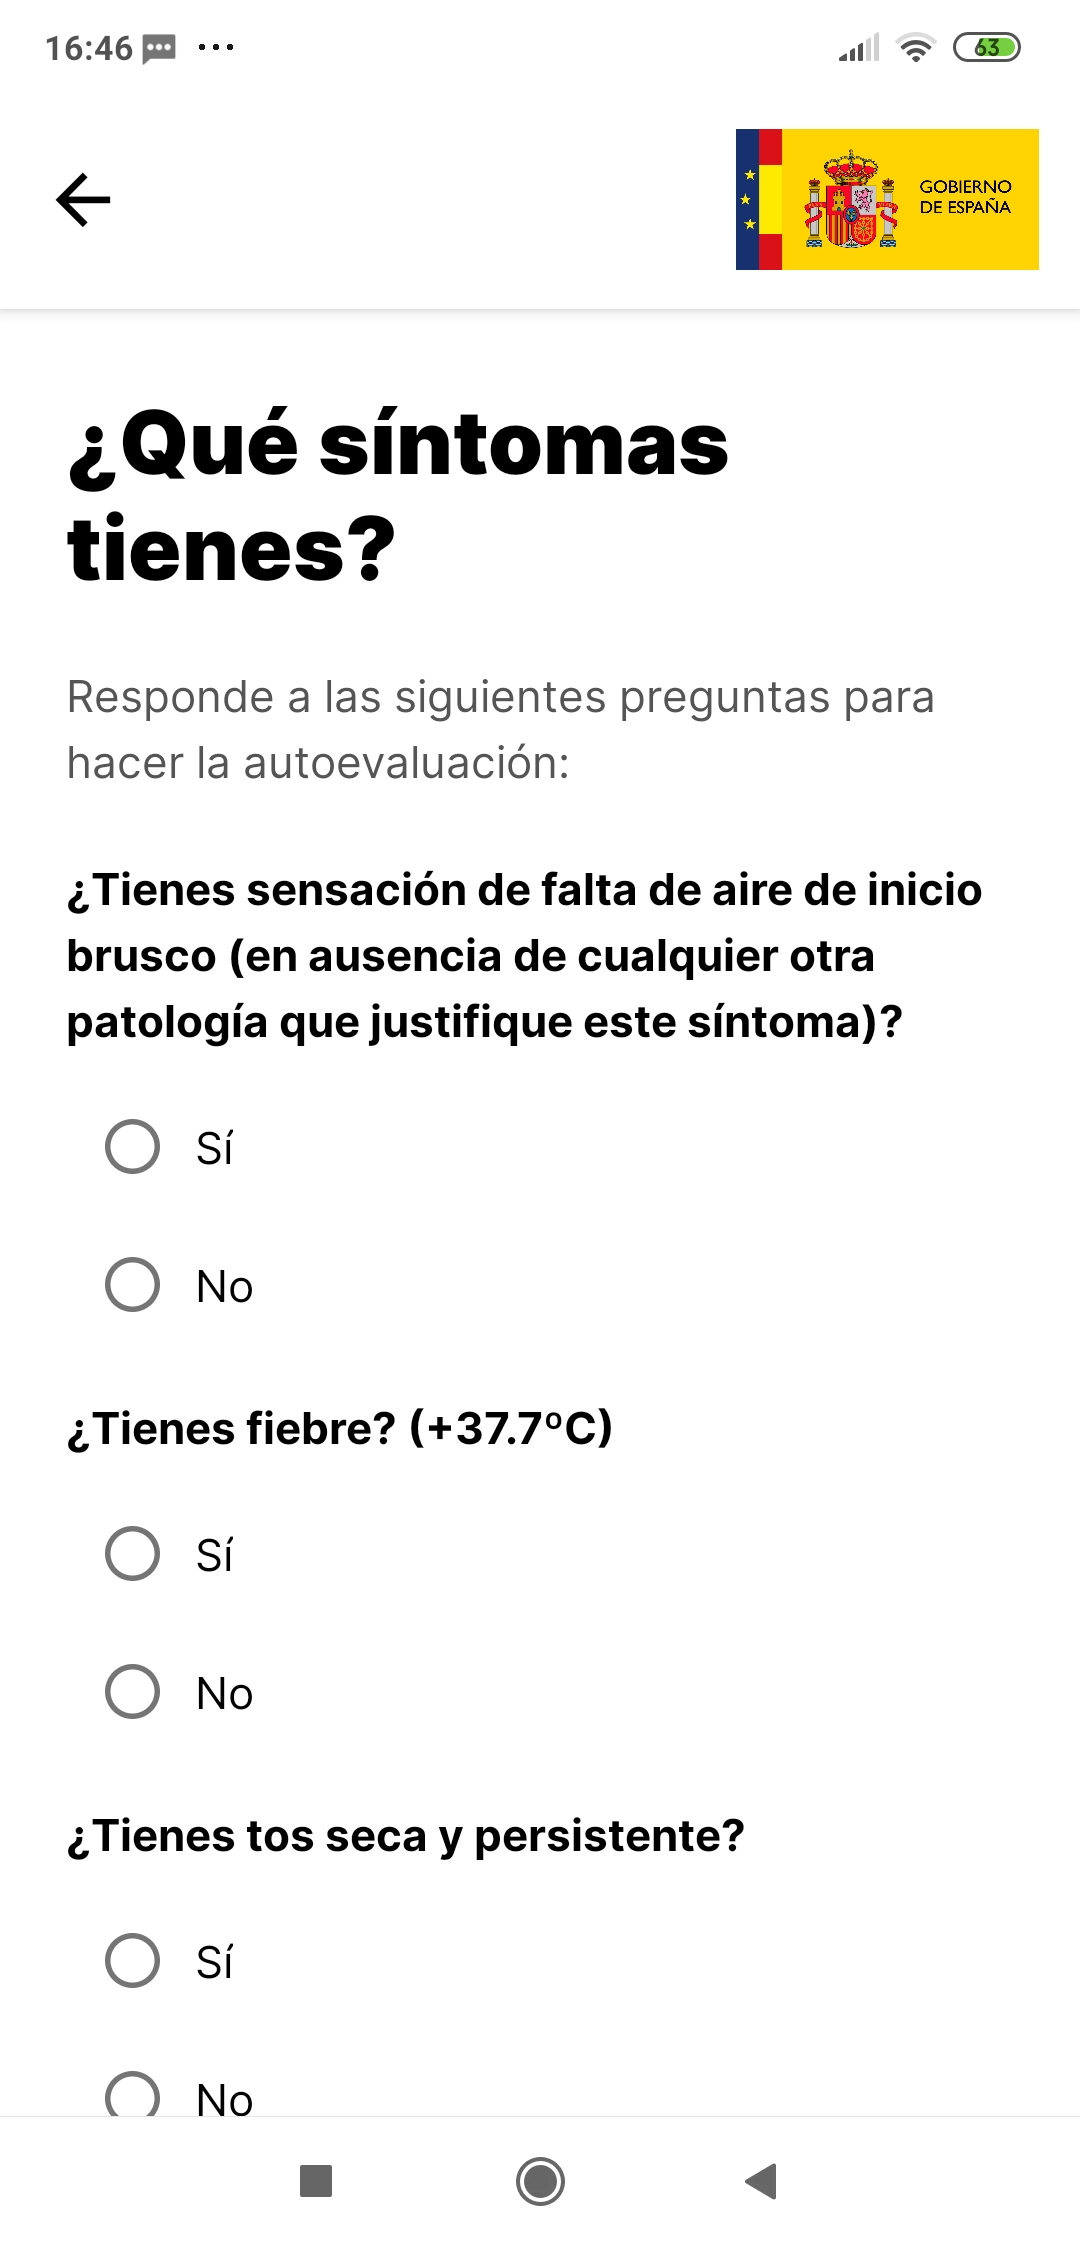
\includegraphics[scale=0.06]{images/discussion/asistencia-covid-2.jpg}
   \end{minipage}
   \begin{minipage}{0.33\textwidth}
     \centering
     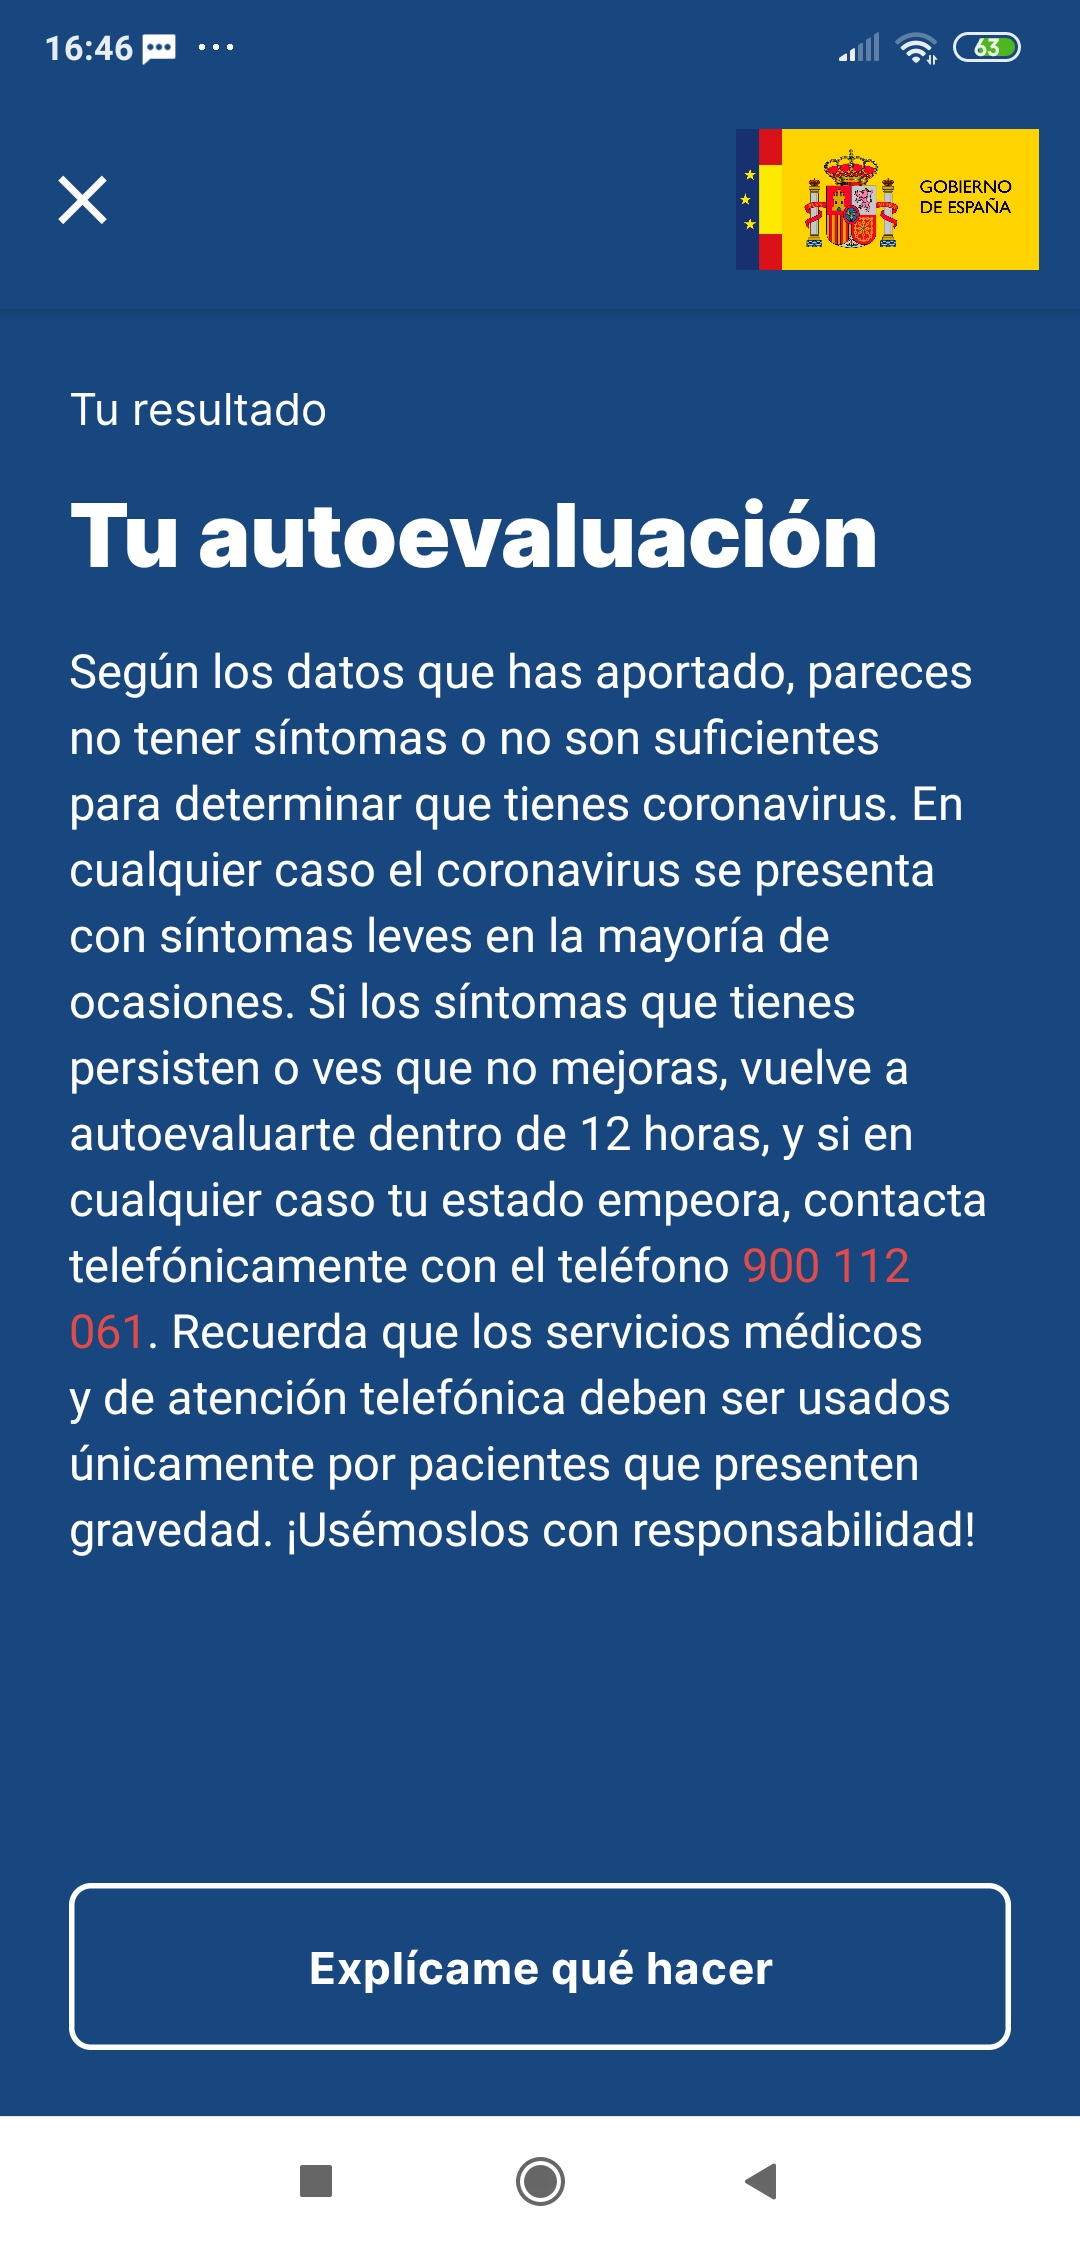
\includegraphics[scale=0.06]{images/discussion/asistencia-covid-3.jpg}
   \end{minipage}
   \caption{Different screens of the application Asistencia COVID-19}
   \label{fig:asistencia-covid-19}
\end{figure}

The analysis of the user interface of the application, makes clear that it was inspired by \textit{CoronaMadrid}, (similarities in the user interface can be shown in Figure \ref{fig:asistencia-covid-19}). One visual element that hold important similarities between those apps are forms, having essentially the same information, with some minor differences; especially in the one for introducing personal details.

%%%%%%%%%%%%%%%%%%%%%%%%%%

%%%%%%%% SECTION 3 %%%%%%%
\section{Discussion of the situation of the current COVID-19 applications}
\label{section:discussion}

Lorem ipsum dolor sit amet, consectetur adipiscing elit. Fusce ultrices nisl in libero aliquet eleifend. Nam nibh leo, egestas non auctor eu, egestas eu libero. Cras sem tortor, pulvinar sed tincidunt et, viverra id ipsum. Suspendisse venenatis pharetra lectus sit amet porta. Cras euismod et tellus in aliquet. Quisque non posuere velit. Vivamus dui tortor, euismod eu imperdiet vel, ornare vel lectus. Vestibulum id ex neque. Curabitur ligula magna, sagittis at pulvinar in, mattis at magna.

%%%%%%%%%%%%%%%%%%%%%%%%%%

%%%%%%%% SECTION 4 %%%%%%%
\section{Conclusions}
\label{section:conclusions}

Lorem ipsum dolor sit amet, consectetur adipiscing elit. Fusce ultrices nisl in libero aliquet eleifend. Nam nibh leo, egestas non auctor eu, egestas eu libero. Cras sem tortor, pulvinar sed tincidunt et, viverra id ipsum. Suspendisse venenatis pharetra lectus sit amet porta. Cras euismod et tellus in aliquet. Quisque non posuere velit. Vivamus dui tortor, euismod eu imperdiet vel, ornare vel lectus. Vestibulum id ex neque. Curabitur ligula magna, sagittis at pulvinar in, mattis at magna.

%%%%%%%%%%%%%%%%%%%%%%%%%%

%%%%%% BIBLIOGRAPHY %%%%%%
\addcontentsline{toc}{section}{References}

\bibliographystyle{acm}
\bibliography{bibliography}
\nocite{*}
%%%%%%%%%%%%%%%%%%%%%%%%%

\end{document}